% Chapter X

\chapter{Trachée} % Chapter title


\label{ch:01-01} % For referencing the chapter elsewhere, use \autoref{ch:name} 

%----------------------------------------------------------------------------------------

% \section{}

La trachée fait suite au larynx, c’est un cylindre de 10 à 12 cm de long et de 1 à 2 cm de diamètre qui se termine par bifurcation en deux bronches principales au niveau du médiastin. La paroi trachéale est formée de trois couches: 
\begin{itemize}
\item La muqueuse de type respiratoire, comporte un épithélium pseudo stratifié composé de cellules ciliées et renfermant des cellules caliciformes qui sécrète le mucus. Le chorion est riche en fibres élastique, en glandes mixtes, en tissu lymphoïde ou la vascularisation est abondante et riche en nerfs La muqueuse a pour rôle entre autre d’empêcher le collapsus de la paroi trachéale pendant la respiration mais aussi le réchauffement, l’humidification et la filtration de l’air respiré
\item La tunique fibrocartilagineuse est constituée d’anneaux cartilagineux dans sa partie antérieure et les bandes musculaires lisses en postérieur lui confèrent sa flexibilité
\item L’adventice un tissus conjonctif riche en vaisseaux et en nerfs.
\end{itemize}

\begin{figure}[h!]
    \begin{minipage}[b]{0.4\linewidth}
        \centering 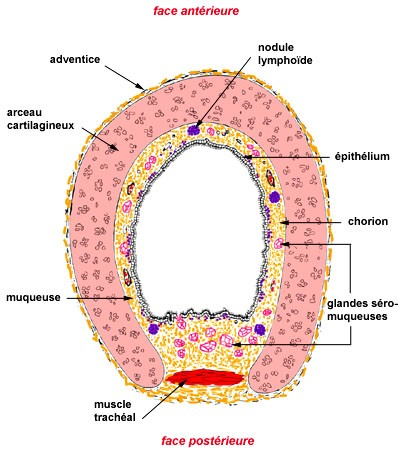
\includegraphics[scale=0.4]{gfx/Trach_esch_mas.jpg}
        \centering \caption{Schémas trachée}
        \label{Trachéeschémas}
    \end{minipage}\hfill
    \begin{minipage}[b]{0.7\linewidth}
        \centering 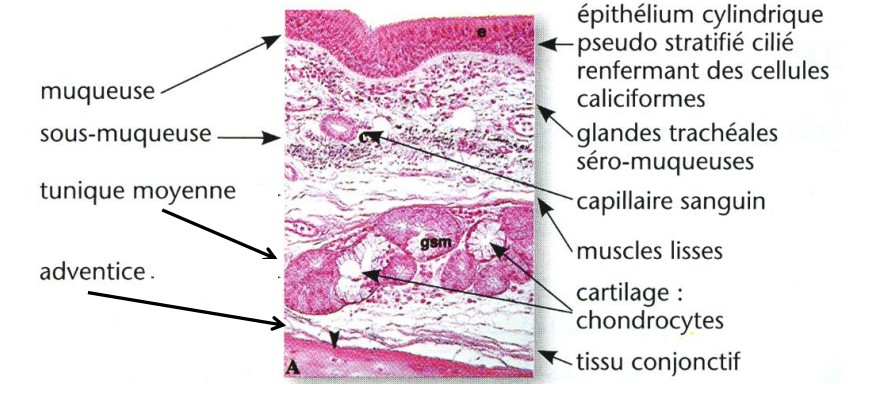
\includegraphics[scale=0.4]{gfx/Trach_ecoupe.jpg}
        \centering \caption{Coupe trachée}
        \label{Trachéecoupe}
    \end{minipage}
\end{figure}

La structure et la fonction de la trachée sont en relation étroite. De forme cylindrique elle assure le passage de l'air durant tout le cycle de la respiration, elle présente aussi, en relation avec son appareil mucociliaire, une fonction de drainage permettant l'élimination des particules inhalées vers le pharynx. (Figure \ref{Trachéeschémas} et Figure \ref{Trachéecoupe})

%------------------------------------------------

% \subsection{Subsection Title}

% Content
